\documentclass[problem]{mcs}

\begin{pcomments}
  \pcomment{TP_disjoint_trees}
  \pcomment{ARM 4/13/14}
\end{pcomments}

\pkeywords{
  tree
  graph
  spanning
}

%%%%%%%%%%%%%%%%%%%%%%%%%%%%%%%%%%%%%%%%%%%%%%%%%%%%%%%%%%%%%%%%%%%%%
% Problem starts here
%%%%%%%%%%%%%%%%%%%%%%%%%%%%%%%%%%%%%%%%%%%%%%%%%%%%%%%%%%%%%%%%%%%%%
\begin{problem}

\begin{figure}[h]
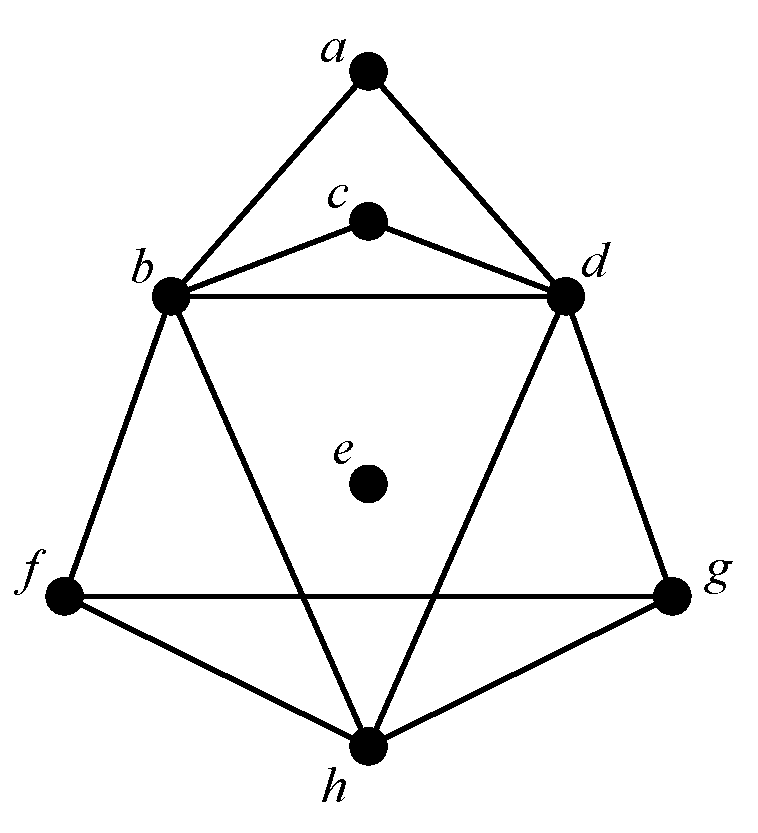
\includegraphics[width=0.4\linewidth]{MQ_coloring}
\caption{The graph $G$.}
\label{fig:spanG}
\end{figure}


\bparts

\ppart How many spanning trees are there for the graph $G$ in
Figure~\ref{fig:spanG}?

\begin{solution}
0 because it is disconnected.
\end{solution}

\ppart For $G-e$, the graph $G$ with vertex $e$ deleted, describe two
spanning trees that have no edges in common.

\begin{solution}
   Edge $\edge{b}{f}$ and all other vertices as leaves; also edge
   $\edge{d}{g}$ and all other vertices as leaves.
\end{solution}

\ppart For $G-e$ with edge $\edge{a}{d}$ deleted, explain why there
cannot be two edge-disjoint spanning trees.

   \hint: Count vertices and edges.

\begin{solution}
There are 7 vertices and 11 edges.  A spanning tree must have 6 edges,
and the 11 edges cannot be partitioned into two blocks of 6.
\end{solution}

\eparts

\end{problem}

%%%%%%%%%%%%%%%%%%%%%%%%%%%%%%%%%%%%%%%%%%%%%%%%%%%%%%%%%%%%%%%%%%%%%
% Problem ends here
%%%%%%%%%%%%%%%%%%%%%%%%%%%%%%%%%%%%%%%%%%%%%%%%%%%%%%%%%%%%%%%%%%%%%

\endinput
